\chapter{Semiconductors}

This will be a brief introduction to physical electronics.  To properly study the field requires both quantum and statistical mechanics.  Perhaps one day I will write up a book on these topics and will then have the background material available to show more of the why.  For now I will attempt to give an understanding of the key concepts and an explanation of how to solve for key values.

\section{Energy Levels}

In electronics we are concerned about three basic types of materials: insulators, semiconductors, and conductors.  Their properties come from the energy gap between their valence\footnote{topmost filled band} (energy level of the valence band is denoted $E_v$) and conduction\footnote{band above the valence band} (energy level of the conduction band is denoted $E_c$) bands, and where the Fermi energy\footnote{A formal discussion is beyond the scope, so I will try to give a simple explanation.  In thermal equilibrium the Fermi energy is the chemical potential, i.e. the amount the energy of the system changes when particles are added or subtracted from it.  It is a crucial element in determining the probability a state contains an electron.  The Fermi energy can also be thought of as the critical energy of the Fermi-Dirac distribution (the energy at which the probability is $0.5$).  Note the Fermi energy is always greater than the energy of the highest filled band.} (denoted $E_f$) lies with respect to them.
\begin{description}
  \item[Conductors] have a small energy gap between the valence and conduction band and the Fermi energy is at or above the level of the conduction band.  Charge carriers are readily available to carry current.  This is how they conduct.
  \item[Semiconductors] have a small to mid sized gap and the Fermi energy lies in this gap.  Charge carriers are not readily available, but can be made to be available by other factors (temperature, electric field, photons, donors/acceptors, etc.).  This ability to conduct or insulate is the source of the name.  We break down semiconductors into different categories: intrinsic and extrinsic.  Extrinsic is then broken down into p or n type.
  \item[Insulators] have a large energy gap between the valence and conduction band and the Fermi energy is between them, though not close to the conduction band.  This means charge carriers are very unlikely available to move and thus carry current.  This is how they insulate.
\end{description}
Quantum theory tells us that the electrons around an atom are in shells that have quantized energy values.  Further, due to the Pauli Exclusion Principle, no two electrons can have the same quantum numbers (n, l, m, s), which also applies in systems of multiple atoms.  As atoms come closer together the shells split so the quantum numbers are unique between them.


%To explain where these energies come from we need to do a brief review of some results from quantum theory.  The total energy of an electron bound to a hydrogen nucleus is given by
%\begin{eqnarray}
%E(n) &=& \frac{-m_eq^4}{8\pi^2\epsilon_0^2\hbar^2n^2}\\
%     &=& \frac{-m_eq^4}{2\epsilon_0^2h^2n^2}
%\end{eqnarray}
%where
%\begin{description}
%  \item[$n$] n is the principle quantum number and takes the values of $\{1, 2, \ldots\}$.
%  \item[$m_e$] mass of an electron ($9.11\times 10^{-31}$ [kg]).
%  \item[$q$] charge of an electron ($1.6\times 10^{-19}$ [C]).
%  \item[$\epsilon_0$] permittivity of free space ($8.85\times 10^{-12}$ [F/m]).
%  \item[$\hbar$] modified Planck's constant ($1.054\times 10^{-34}$ [J-s]), which is just Planck's constant divided by $2\pi$.
%  \item[$h$] Planck's constant ($6.625\times 10^{-34}$ [J-s]).
%\end{description}




\section{Intrinsic Semiconductors}

Intrinsic semiconductors are materials that semiconduct in and of themselves.  They come in two varieties, elemental (Si, Ge) and compound (GaAs, InP, etc.), which simply tells you if the material is an element or a compound (made of several elements).  Elemental semiconductors come from column IVa of the periodic table, see Table~\ref{t-PeriodicTable}, as they have half their outer s and p sub-shells filled.  Compound intrinsic semiconductors are compounds that behave like elemental intrinsic semiconductors, as they are formed by bonding elements on either side of column IVa.  I will mostly discuss elemental, though the principles are the same for compound intrinsic semiconductors.

\begin{table}
\caption{Semiconductors in the Periodic Table and Intrinsic Semiconductor Properties}\label{t-PeriodicTable}\label{T:IntSemi}
\begin{tabular}{cc}
\begin{tabular}{|c|c|c|c|c|c|}
\NoSide{IB}    & \NoSide{IIB}   & \NoSide{IIIA}  & \NoSide{IVA}   & \NoSide{VA}    & \NoSide{VIA}   \\
\cline{3-6}
\NoSide{}      & \RtSide{}      & 5              & 6              & 7              & 8              \\
\NoSide{}      & \RtSide{}      & B              & C              & N              & O              \\
\cline{3-6}
\NoSide{}      & \RtSide{}      & 13             & 14             & 15             & 16             \\
\NoSide{}      & \RtSide{}      & Al             & Si             & P              & S              \\
\hline
29             & 30             & 31             & 32             & 33             & 34             \\
CU             & Zn             & Ga             & Ge             & As             & Se             \\
\hline
47             & 48             & 49             & 50             & 51             & 52             \\
Ag             & Cd             & In             & Sn             & Sb             & Te             \\
\hline
79             & 80             & 81             & 82             & 83             & 84             \\
Au             & Hg             & Tl             & Pb             & Bi             & Po             \\
\hline
\end{tabular}
%\end{table}
%\begin{table}
%\caption{Properties of intrinsic semiconductors.}\label{T:IntSemi}
&
\begin{tabular}{lccc}
Material          & Symbol & $E_g$[$eV$] & B[$cm^{-3}K^{-3/2}$]\\\hline
%Gallium Nitride   & GaN    & 3.5         & \\
%Gallium Phosphide & GaP    & 2.26        &                      \\
Gallium Arsenide  & GaAs   & 1.42        & $2.10\times 10^{14}$ \\
Germanium         & Ge     & 0.66        & $1.66\times 10^{15}$ \\
Silicon           & Si     & 1.12        & $5.23\times 10^{15}$ \\
\end{tabular}
\\ \end{tabular}
\end{table}

%Silicon, Si - the most common semiconductor, atomic number 14, energy gap Eg = 1.12 eV - indirect bandgap; crystal structure - diamond, lattice constant 0.543 nm, atomic concentration 5x1022 atoms/cm-3, index of refraction 3.42, density 2.33 g/cm3, dielectric constant 11.7, intrinsic carrier concentration 1.02 x 1010 cm-3, mobility of electrons and holes at 300 K: 1450 and 500 cm2/V-s, thermal conductivity 1.31 W/cm-oC, thermal expansion coefficient 2.6 x 10-6 1/oC, melting point 1414 oC; excellent mechanical properties (MEMS applications); single crystal Si can be processed into wafers up to 300 mm in diameter.

%Ge, C, Sb.


%Gallium Arsenide, GaAs - After silicon second the most common semiconductor, energy gap Eg = 1.43 eV, direct bandgap; crystal structure - zinc blend, lattice constant 5.65 Ang., index of refraction 3.3, density 5.32 g/cm3, dielectric constant 12.9, intrinsic carrier concentration 2.1 x 106 cm-3, mobility of electrons and holes at 300 K - 8500 and 400 cm2/V-s, thermal conductivity 0.46 W/cm-oC, thermal expansion coefficient 6.86 x 10-6 oC-1; thermally unstable above 600 oC due to As evaporation; does not form sufficient quality native oxide; mechanically fragile; due to direct bandgap commonly used to fabricate light emitting devices; due to higher electron and hole mobilities, also foundation of the variety of high-speed electronic devices; bandgap can be readily engineered by forming ternary compounds based on GaAs, e.g. AlGaAs.

%Gallium Nitride, GaN - wide bandgap III-V semiconductor with direct bandgap 3.5 eV wide; among very few semiconductors capable of generating blue radiation, GaN is used for blue LEDs and lasers; intrinsically n-type semiconductor but can be doped p-type; GaN is formed as an epitaxial layer; Lattice mismatch remains a problem, creating a high defect density. Incorporation of Indium (InxGa1-xN) allows control of emission from green to violet (high and low In content respectively). GaN can also be used in UV detectors that do not respond to visible light. GaN has a Wurtzite(W) or Zinc Blend(ZB) crystal structure. Lattice constant [A] 3.189(W) 5.186(ZB); Density[g/cm3] 6.15(W) 6.15(ZB); Atomic concentration [cm-3] 8.9 x 1022(W) 8.9 x 1022(ZB); Melting point [oC] 2,500(W) 2,500(ZB); Thermal conduct.[W/cm oC] 1.3(W) 1.3(W); Thermal expansion coefficient[oC-1] ~1x10-6; Dielectric constant (static) 8.9(W) 9.7(ZB); Refractive index 2.4(W) 2.3(ZB);

%GaP - Crystal structure zinc blend; Lattice constant [A] 5.45; Density [g/cm3] 4.14; Atomic concentration [cm-3] 4.94 x 1022; Melting point [oC] 1457; Thermal conductivity [W/cm oC] 1.1; Thermal expansion coefficient[1/oC] 4.65x10-6; Dielectric constant 11.1; Refractive index 3.02; Energy gap [eV] 2.26; Type of energy gap: direct; Electron mobility [cm2/V sec] 250; Hole mobility [cm2/V sec] 150;

% CdSe, CdTe, CdHgTe, ZnS

%Silicon carbide, SiC - semiconductor featuring energy gap Eg = 2.9 -3.05 eV (wide bandgap semiconductor), indirect bandgap; SiC can be obtained in several polytypes- most common hexagonal in the form of either 4H or 6H polytypes; parameters vary depending on polytype; Intrinsically n-doped; p-type doping and n-type conductivity control can be obtained by doping with aluminum and nitrogen respectively. SiC features higher than Si and GaAs electron saturation velocity; excellent semiconductor but difficult and expensive to fabricate single-crystal wafers; excellent for high power, high temperature applications; SiC is closely lattice matched to GaN, has a thermal expansion coefficient close to GaN, and is available in both conductive and semi-insulating substrates. Thus it is often used as a substrate for GaN epitaxial layers. SiC wafers 75 mm in diameter are available commercially.
%Crystal Structure 3C-SiC (cubic) 6H-SiC (hexagonal)
%Lattice constant [A] 4.36 3.08
%Thermal conductivity [W/cm oC] 5
%Melting point sublimes > 2,100 oC
%Dielectric constant 9.7
%Energy gap [eV] 2.3 3.03
%Electron Drift Mobility [cm2/V sec] 800 400
%Hole Drift Mobility [cm2/V sec] 40 100



%Equations used to calculate Direct Energy Gap
%AlxIn1-xP 1.34 + 2.23x
%AlxGa1-xAs 1.424 + 1.247 (x<0.45)
%1.424 + 1.087x + 0.438x2
%AlxIn1-xAs 0.36 + 2.35x + 0.24x2
%AlxGa1-xSb 0.73 + 1.10x + 0.47x2
%AlxIn1-xSb 0.172 + 1.621x + 0.43x2
%GaxIn1-xP 1.34 + 0.511x + 0.6043x2
%(0.49
%GaxIn1-xAs 0.356 + 0.7x + 0.4x2
%GaxIn1-xSb 0.172 + 0.165x + 0.413x2
%GaPxAs1-x 1.424 + 1.172x + 0.186x2
%GaAsxSb1-x 0.73 - 0.5x + 1.2x2
%InPxAs1-x 0.356 + 0.675x + 0.32x2
%InAsxSb1-x 0.18 - 0.41x + 0.58x2
%Source: Swaminathan, V; Macrander, A. T.; Materials Aspects of GaAs and InP based Structures. 1991.


\begin{wrapfigure}{r}{0.4\textwidth}
%\vspace*{-.45in}
\begin{center}
\caption{Silicon crystal structure}
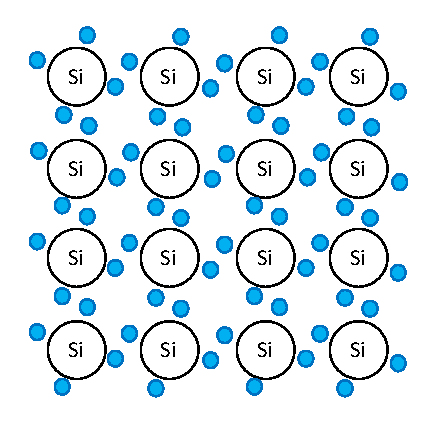
\includegraphics[width=0.35\textwidth]{semiconductors_pure}\label{f-semiconductor-pure}
\end{center}
\end{wrapfigure}

These are (and must be) pure materials, as even a small amount of impurities will cause them not to work.  Most modern semiconductors are extrinsic\footnote{This is due to the excessive cost and difficulty of making a pure or nearly pure material.}, so I will just give a brief overview.  At room temperature, Fermi-Dirac statistics shows the gap between valence and conduction band must be on the order of 1 electron volt or less.  Several materials meet this requirement, such as gallium arsenide (GaAs, 1.42 eV), Silicon (Si, 1.12 eV), and Germanium (Ge, 0.66 eV).  The electrons promoted to the conduction band leave behind holes in the valence band, and current is carried by both the flow of electrons in the conduction band and holes in the valence band.  The flow of the electron-hole pairs (in opposite directions) is the mechanism of current.  Essentially the electron-hole movement is the same for extrinsic semiconductors also, but for extrinsic semiconductors these need not be equal (and are not).

The number of electrons available in the conduction band is  given by
\begin{eqnarray}
n_e &=& 2\left(\frac{2\pi m^*_nkT}{h^2}\right)^{\frac{3}{2}}e^{\left(\frac{-(E_c-E_f)}{2kT}\right)}\\
&=&BT^{\frac{3}{2}}e^{\left(\frac{-(E_c-E_f)}{2kT}\right)}
\end{eqnarray}



Since the number of electrons in the conduction band and the number of holes in the valence band are equal in an intrinsic semiconductor, we will just consider the density of the intrinsic carriers (either electron or hole), $n_i$.
\begin{eqnarray}
n_i &=& BT^{\frac{3}{2}}e^{\left(\frac{-E_g}{2kT}\right)}
\end{eqnarray}
The temperature in Kelvin is $T$.  The values of $B$ and $E_g$ are dependent on the material, and are provided for our top three intrinsic materials in Table~\ref{T:IntSemi}.The Boltzmann constant, $k$, is $86\times 10^{-6}$[$eV/K$].

\begin{example}
What is the carrier density of Germanium at room temperature?

Answer:

Room temperature is not a well defined term, meaning it is not a set temperature.  Roughly it could vary from $65^\circ$F to $85^\circ$F, or in kelvin, from 291K to 303K.  For ease of calculation, we will choose 300K to be room temperature.
\begin{eqnarray}
n_i
&=& BT^{\frac{3}{2}}e^{\left(\frac{-E_g}{2kT}\right)} \\
&=& 1.66\times 10^{15}\cdot 300^{\frac{3}{2}}e^{\left(\frac{-0.66}{2\cdot 86\times 10^{-6} \cdot 300}\right)}\\
&\approx & 2.40\times 10^{13} [cm^{-3}]
\end{eqnarray}
\end{example}

To make life easier in calculating this, I usually use a small SciLab program, see Code~\ref{code:intrinsicCarriers}.

\SciLab{SciLab code to calculate intrinsic carrier density.}{code:intrinsicCarriers}{IntrinsicCarriers.sce}

\section{Extrinsic Semiconductors}

Extrinsic semiconductors are made by adding an impurity into the crystallin structure that is chosen to provide an extra electron above the valence band (a donor or n type), or to provide a deficiency of electrons (an acceptor or p type).  Since the charge carriers (electrons and holes) are no longer balanced, we need to be able to calculate how many of them there are.  A basic relationship is
\begin{eqnarray}
n_e n_h &=& n_i^2 \label{eq:extrinsiccarrierdensity}
\end{eqnarray}
where $n_e$ is the thermal equilibrium concentration of free electrons, $n_h$ is the thermal equilibrium concentration of holes, and $n_i$ is the intrinsic carrier density.  Provided the concentration of the dopant is greater than the intrinsic carrier density, we can approximate the number of carriers of the type provided by the dopant by the concentration of the dopant.  We will denote the dopant concentration by $N_n$ for n type materials and $N_p$ for p type materials.

%A p-type wafer is usually doped with Boron, although Gallium can also be used (rare). P+ wafers are heavily doped and typically have resistances of <1 Ohm/cm2. P+ wafers are often used for Epi substrates. P- wafers are lightly doped with typical resistances of >1 Ohm/cm2. The most common crystal orientations for P-type wafers are {100} and {111}.

%N-type wafers are doped with Phosphorus, Antimony, or Arsenic. N+ wafers are heavily doped with resistances <1 Ohm/cm2. N- wafers are lightly doped with resistances >1 Ohm/cm2.

%Resistivity is very important to good electronic devices and for growing uniform thermal oxides. High resistivity silicon can only be produced using the Float Zone (FZ) crystal growth method, which does not use a crucible during crystal growth. The Czochralski (CZ) method uses a quartz crucible during crystal growth, and oxygen from the crucible unintentionally dopes the material. The oxygen dopant behaves as an n-type impurity and impedes high resistivity. Low resistivity n-type material is achieved using Arsenic doping.

%Wafer flats in relation to doping



\subsection{P Type Semiconductors}

\begin{figure}
\begin{center}
\caption{P Type Silicon crystal structure}\label{f-semiconductor-p}
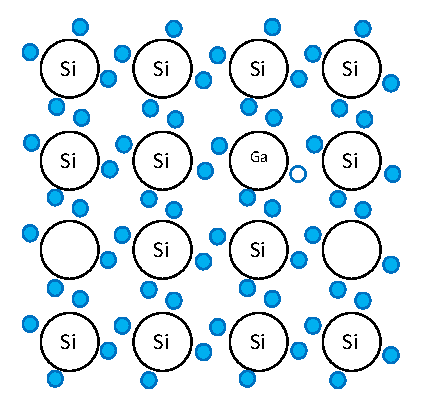
\includegraphics{semiconductors_p}
\end{center}
\end{figure}
If an element like gallium or boron is doped, which has only 3 electrons in its outer shell of up to 8, into the crystallin structure of say silicon, which has 4 electrons in its outer shell of 8, a gap in the bonding is formed, see Figure~\ref{f-semiconductor-p}.  The outer shell of the gallium and the bonded silicon is just one shy of completing and thus it is already free to conduct a hole by stealing an electron from a neighbor.  In terms of energy bands, the energy of this ``hole'' (usually denoted $E_a$) is very close to (but above) the energy of the valence band.  The Fermi energy is thus close to the valence band, which means there will not be lots of free electrons, so the only free carriers are these holes\footnote{In truth the hole is the spot where the electron is missing (and thus not an actual thing), but since this means that the atom that is missing it is ionized (positive in the case of a lack of an electron), it appears that a positive charge is flowing.  This is governed by statistical mechanics and so it is not possible to track the actual electron.  Like it or not, holes are a reasonable description of how the charge is carried.}.

\subsection{N Type Semiconductors}
\begin{figure}
\begin{center}
\caption{N Type Silicon crystal structure}\label{f-semiconductor-n}
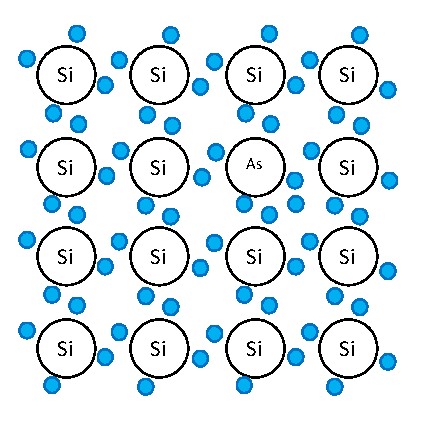
\includegraphics{semiconductors_n}
\end{center}
\end{figure}



